\documentclass[oneside]{book}
\let\cleardoublepage\clearpage 
% \setlength{\textwidth}{700pt}% the default is 390pt so increase by 40pt

\usepackage{graphicx}
% \usepackage[legalpaper, margin=0.1cm]{geometry}

\usepackage[top=0.5cm, left=0cm,right=5cm]{geometry}
\pagenumbering{gobble}
\centering
\begin{document}
\begin{tabular}{l@{\hskip -0.0in}c@{\hskip -0.0in}c@{\hskip -0.0in}c}
% \renewcommand{\arraystretch}{-3.8}
\vspace{-0.2cm}
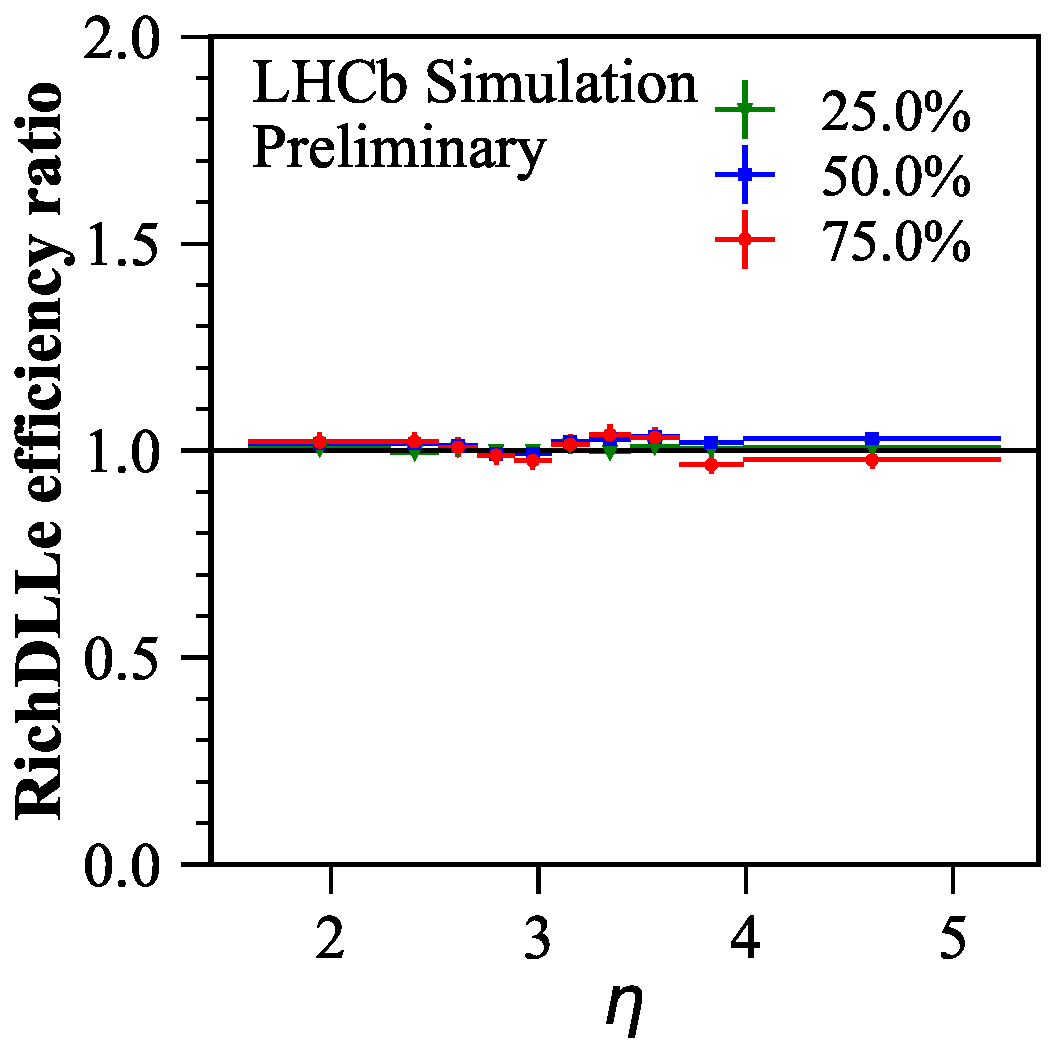
\includegraphics[width=0.3\linewidth]{eff_ratio_RichDLLe_vs_Brunel_ETA_at_[0.05, 0.1, 0.25, 0.5, 0.75, 0.9, 0.95].pdf} &
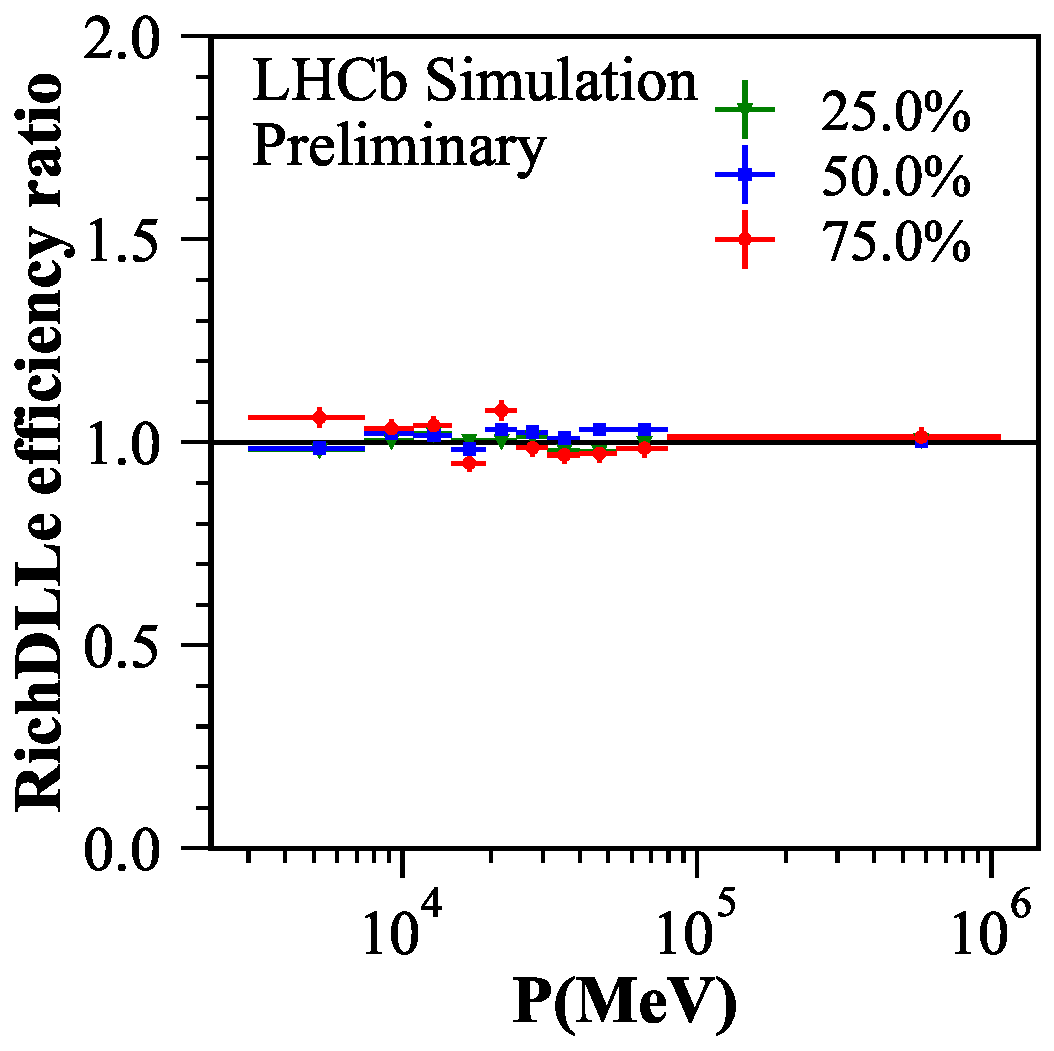
\includegraphics[width=0.3\linewidth]{eff_ratio_RichDLLe_vs_Brunel_P_at_[0.05, 0.1, 0.25, 0.5, 0.75, 0.9, 0.95].pdf} &
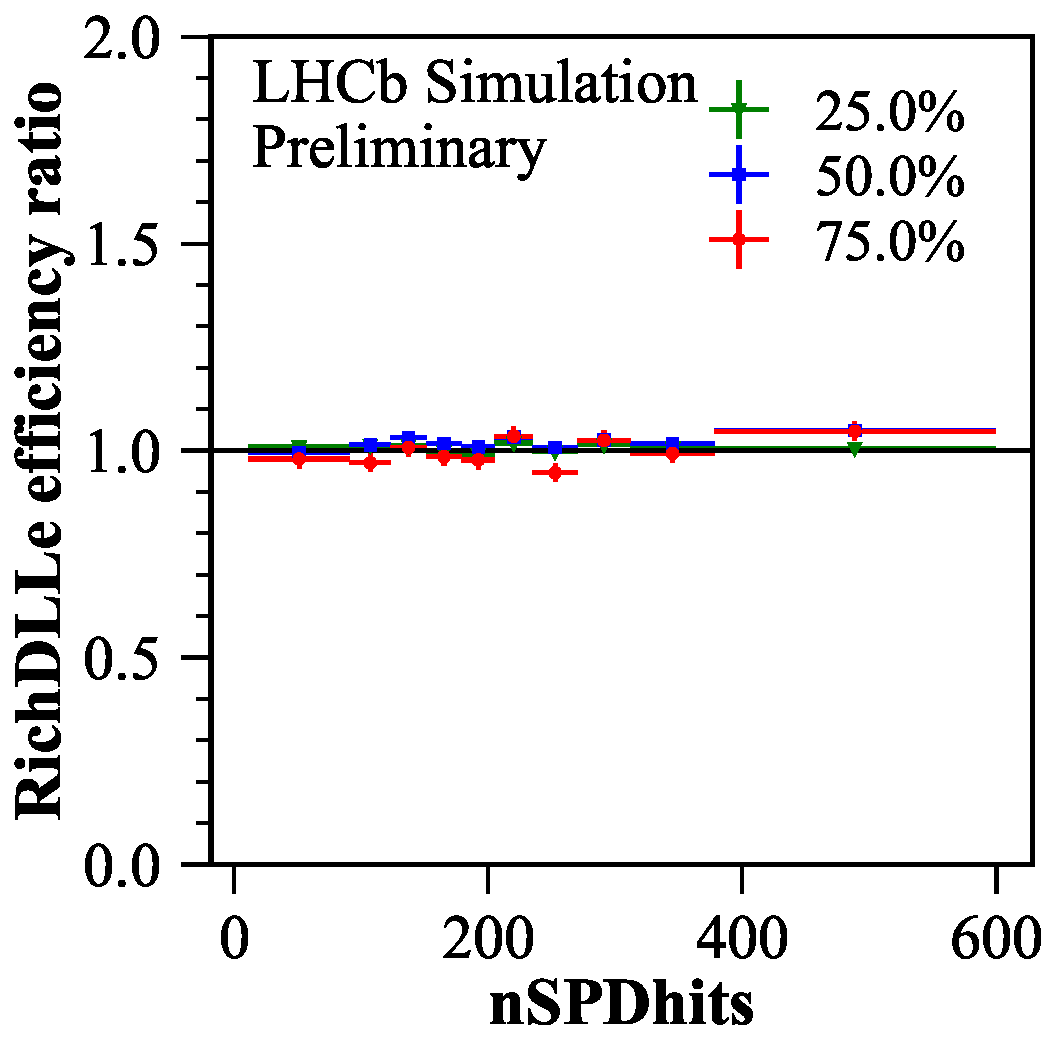
\includegraphics[width=0.3\linewidth]{eff_ratio_RichDLLe_vs_nSPDhits_at_[0.05, 0.1, 0.25, 0.5, 0.75, 0.9, 0.95].pdf} &
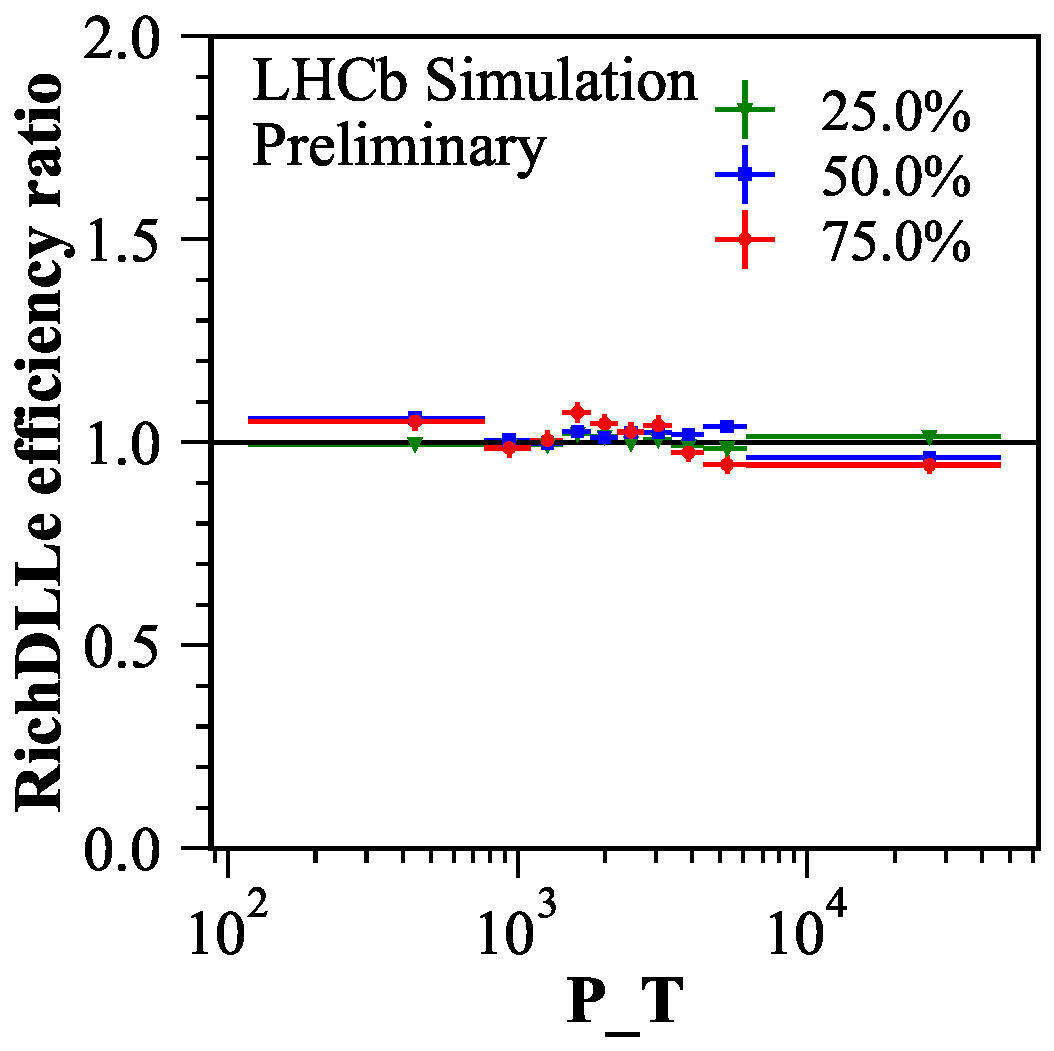
\includegraphics[width=0.3\linewidth]{eff_ratio_RichDLLe_vs_P_T_at_[0.05, 0.1, 0.25, 0.5, 0.75, 0.9, 0.95].pdf}\\
\vspace{-0.2cm}
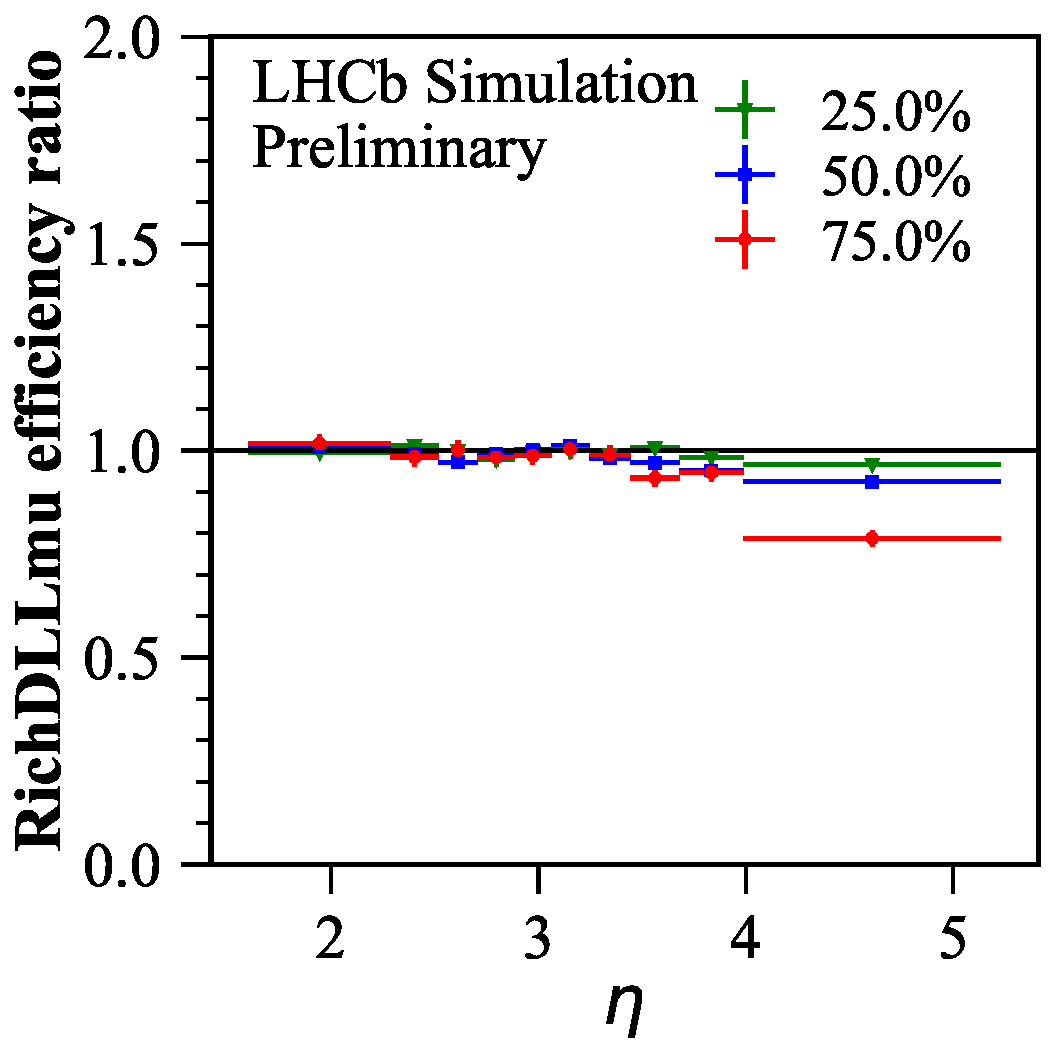
\includegraphics[width=0.32\linewidth]{eff_ratio_RichDLLmu_vs_Brunel_ETA_at_[0.05, 0.1, 0.25, 0.5, 0.75, 0.9, 0.95].pdf} &
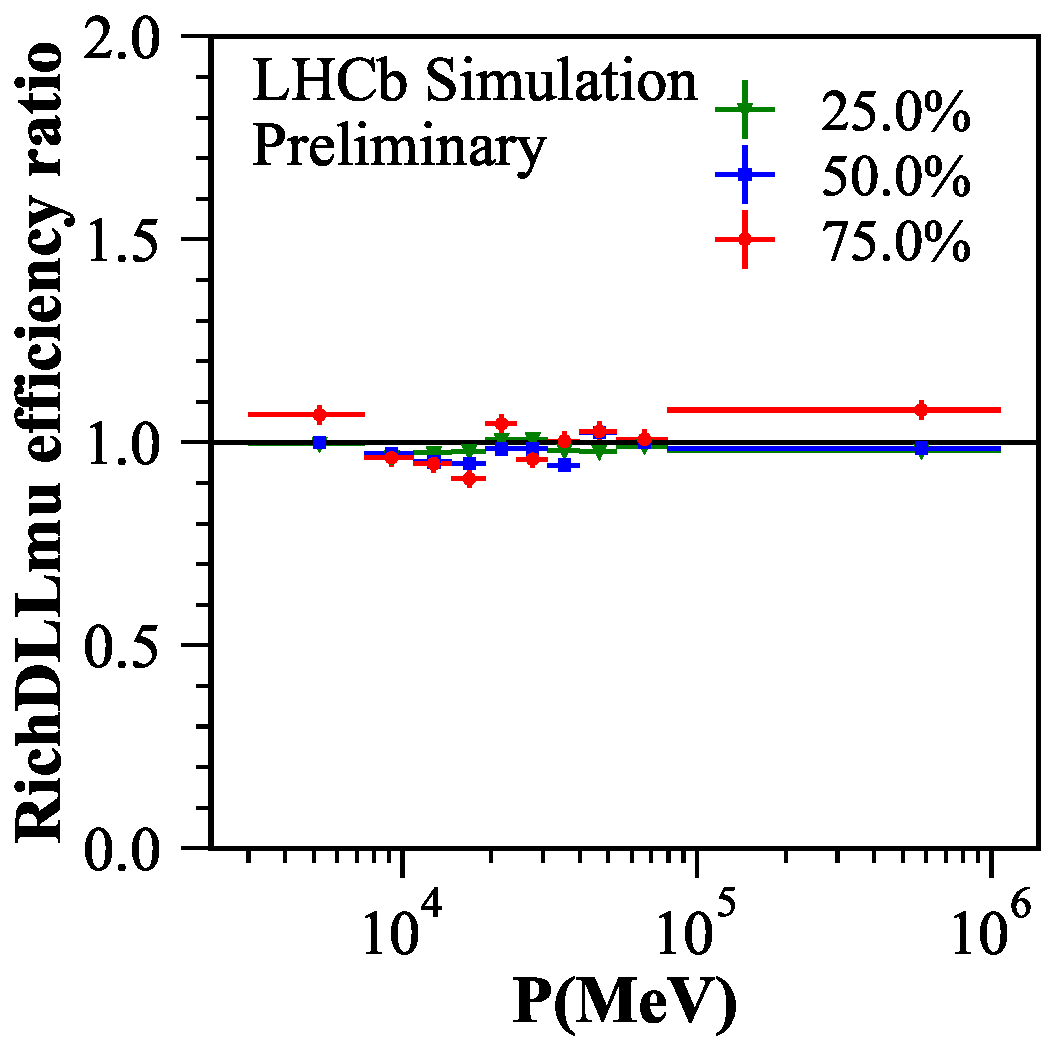
\includegraphics[width=0.32\linewidth]{eff_ratio_RichDLLmu_vs_Brunel_P_at_[0.05, 0.1, 0.25, 0.5, 0.75, 0.9, 0.95].pdf} &
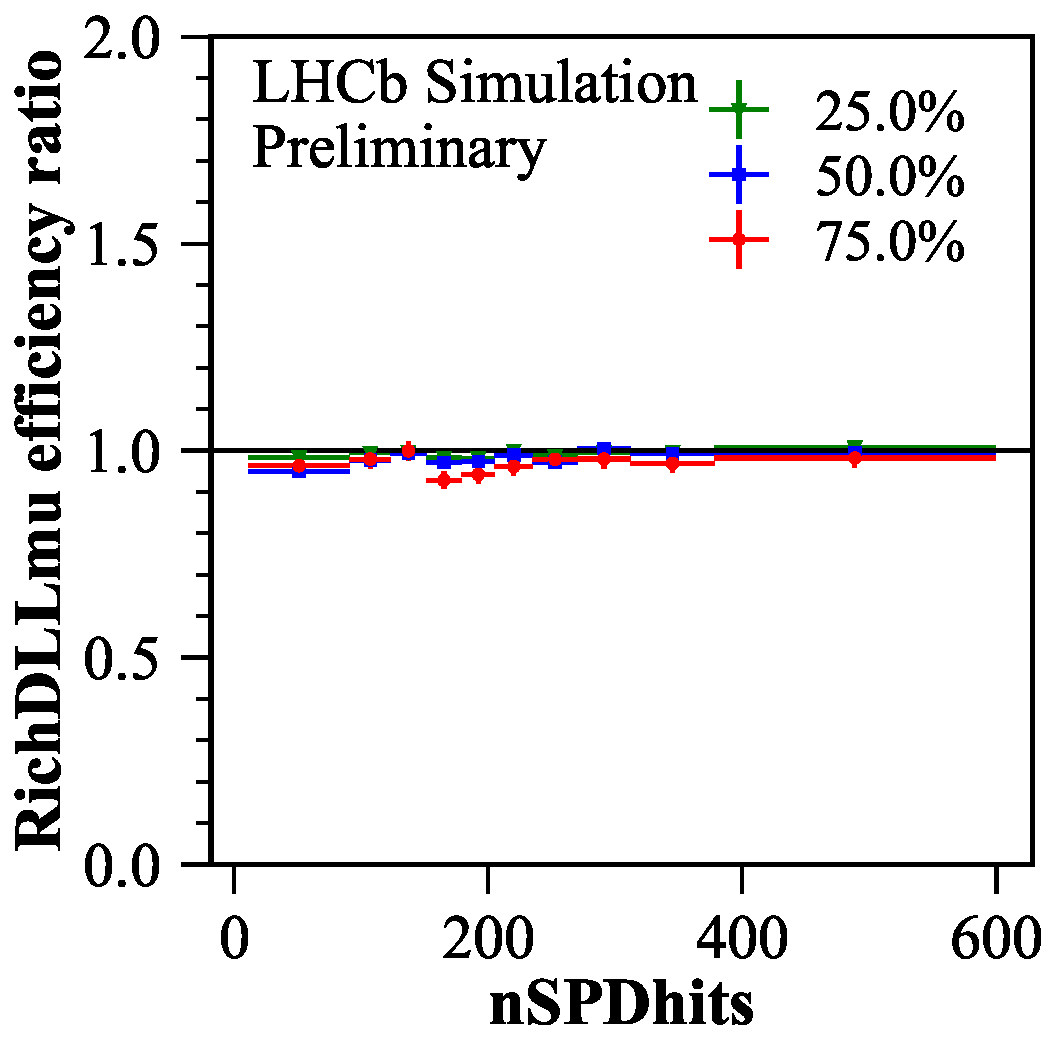
\includegraphics[width=0.32\linewidth]{eff_ratio_RichDLLmu_vs_nSPDhits_at_[0.05, 0.1, 0.25, 0.5, 0.75, 0.9, 0.95].pdf} &
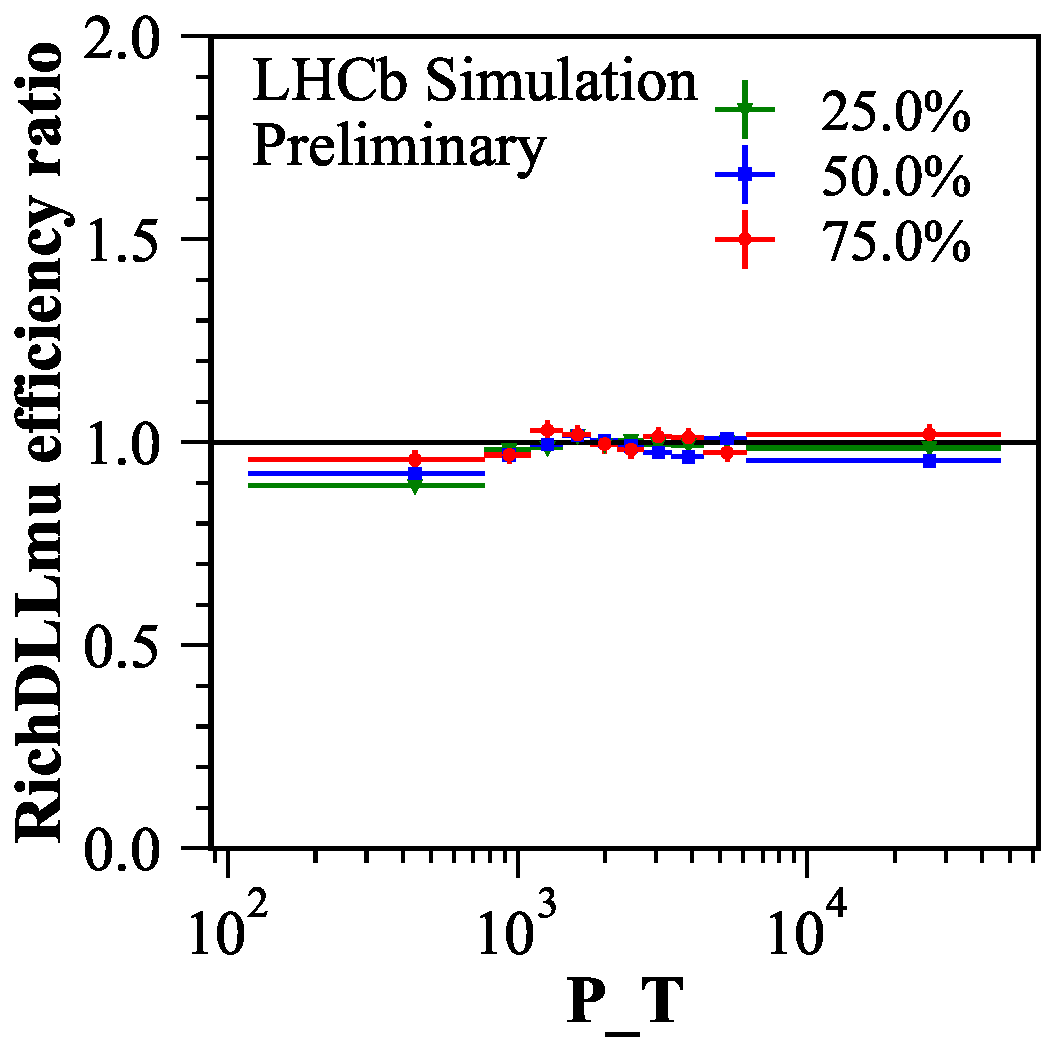
\includegraphics[width=0.32\linewidth]{eff_ratio_RichDLLmu_vs_P_T_at_[0.05, 0.1, 0.25, 0.5, 0.75, 0.9, 0.95].pdf}\\
\vspace{-0.2cm}
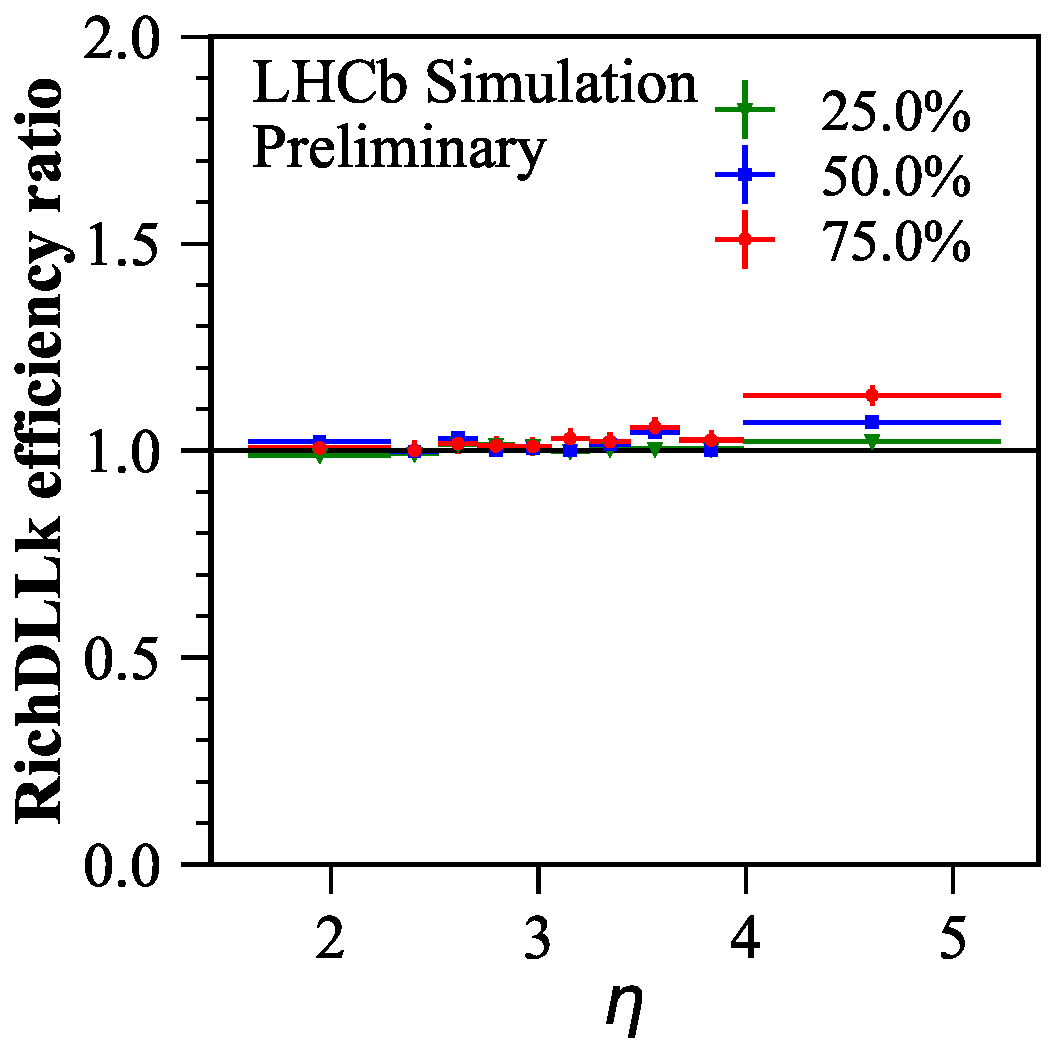
\includegraphics[width=0.32\linewidth]{eff_ratio_RichDLLk_vs_Brunel_ETA_at_[0.05, 0.1, 0.25, 0.5, 0.75, 0.9, 0.95].pdf} &
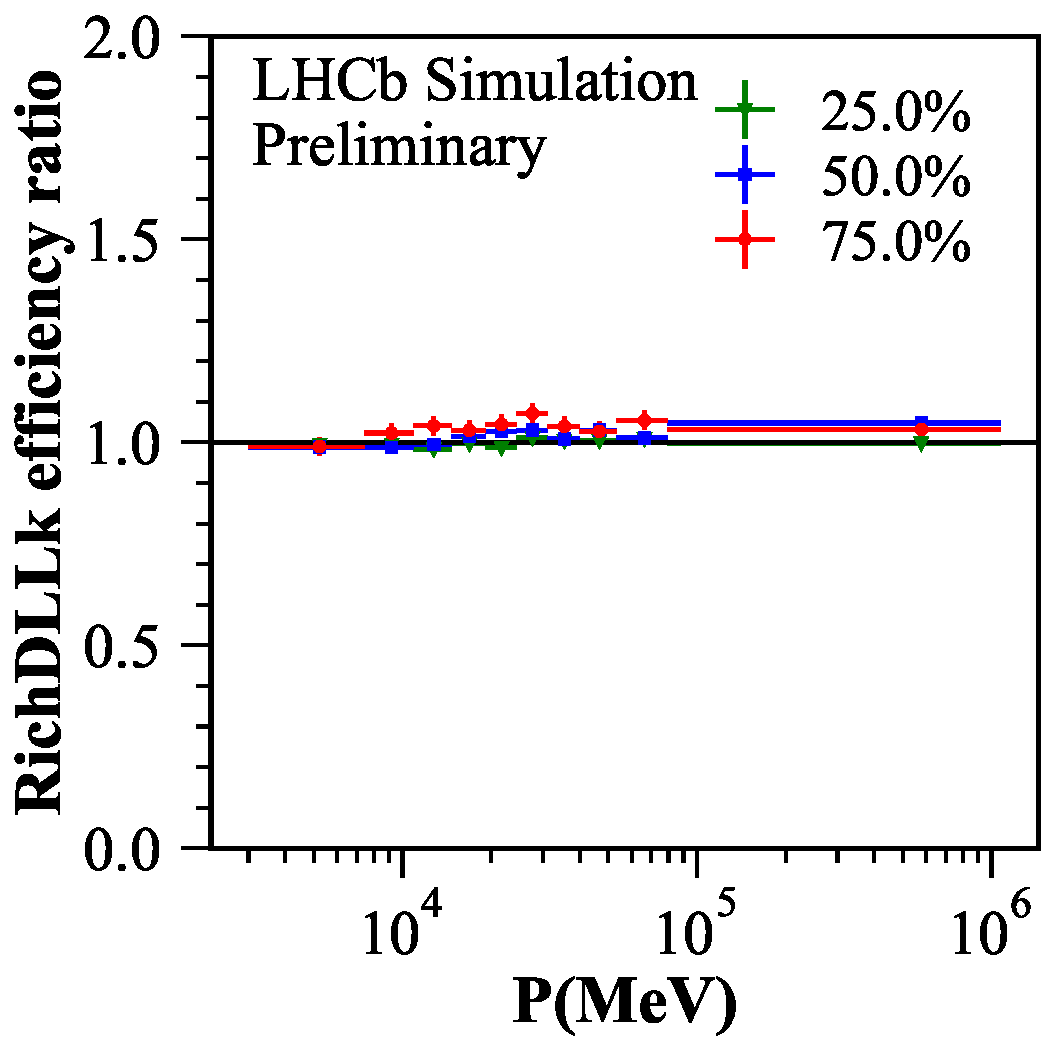
\includegraphics[width=0.32\linewidth]{eff_ratio_RichDLLk_vs_Brunel_P_at_[0.05, 0.1, 0.25, 0.5, 0.75, 0.9, 0.95].pdf} &
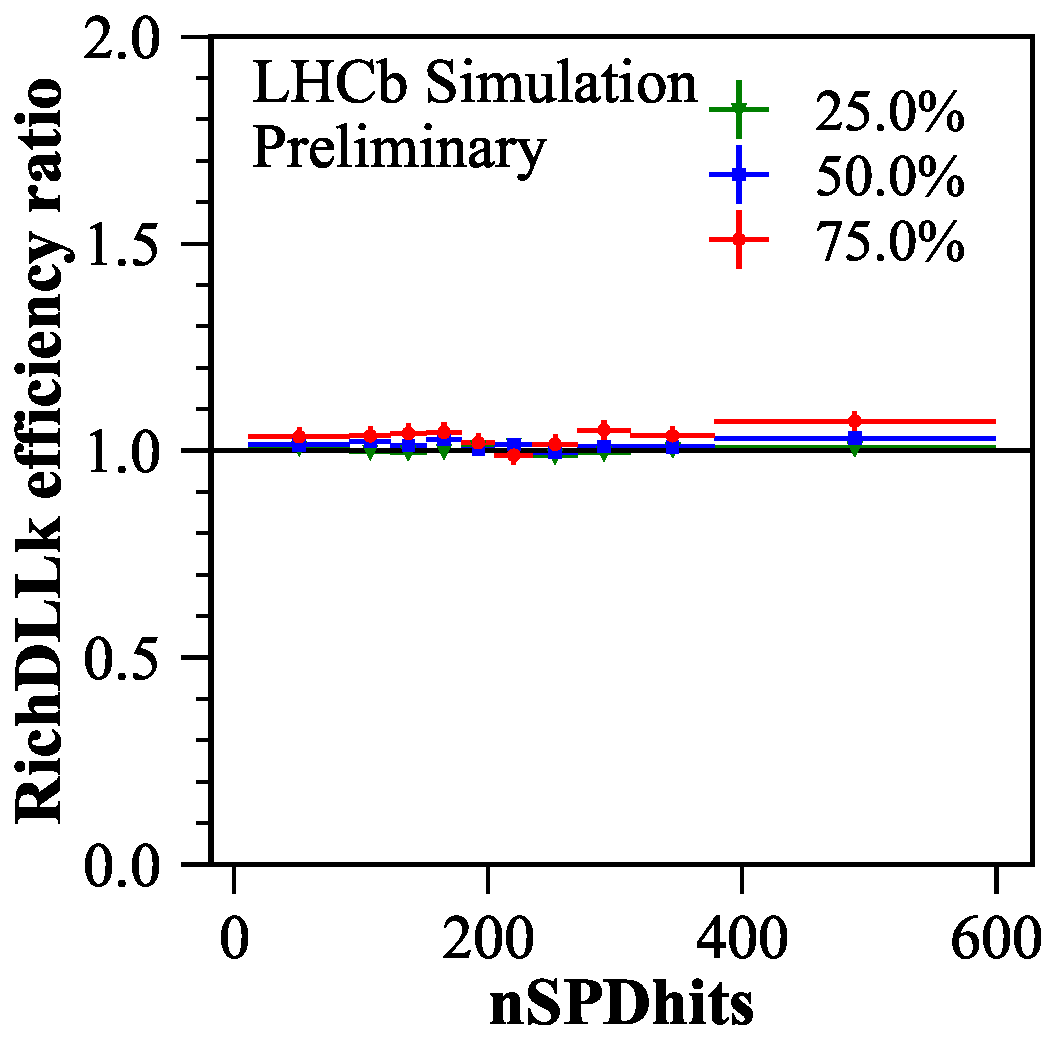
\includegraphics[width=0.32\linewidth]{eff_ratio_RichDLLk_vs_nSPDhits_at_[0.05, 0.1, 0.25, 0.5, 0.75, 0.9, 0.95].pdf}  &
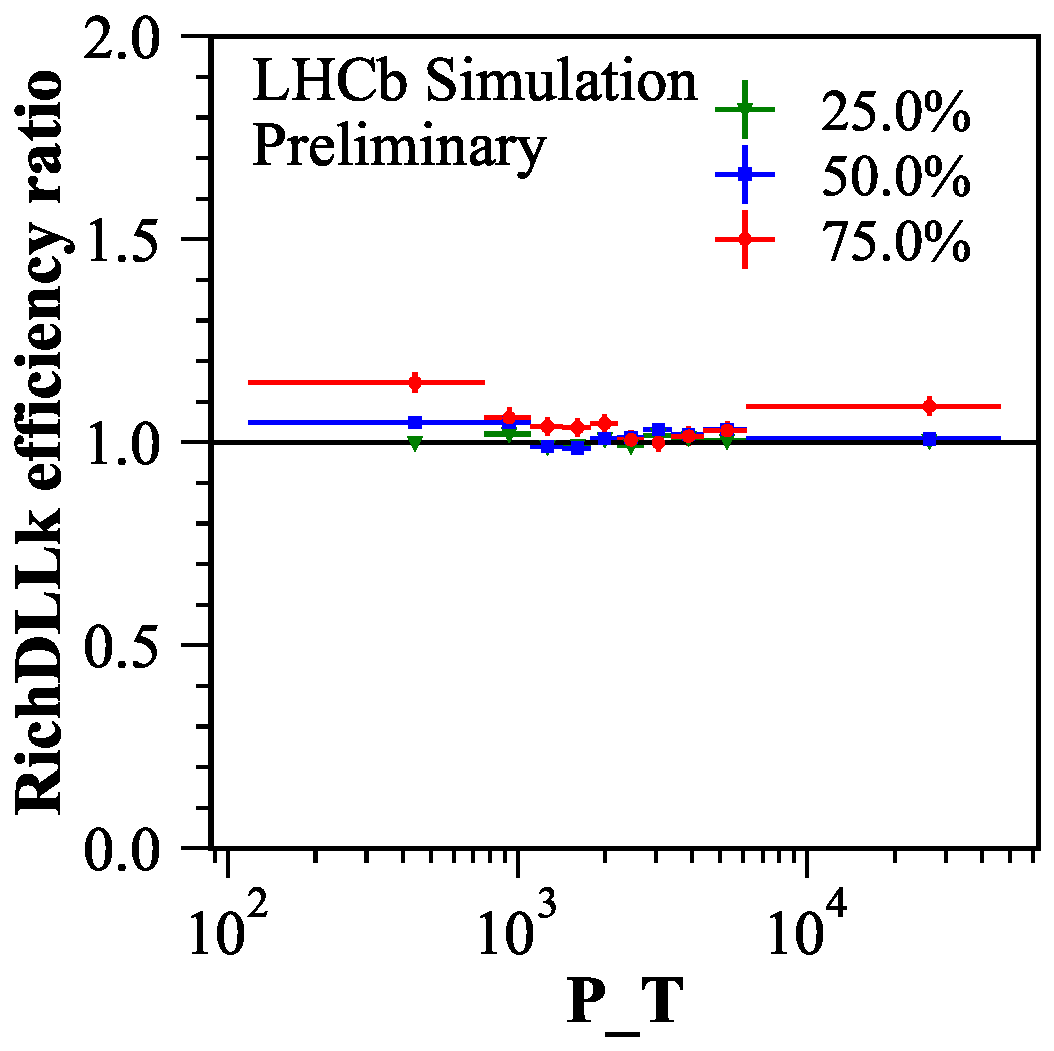
\includegraphics[width=0.32\linewidth]{eff_ratio_RichDLLk_vs_P_T_at_[0.05, 0.1, 0.25, 0.5, 0.75, 0.9, 0.95].pdf}\\
\vspace{-0.2cm}
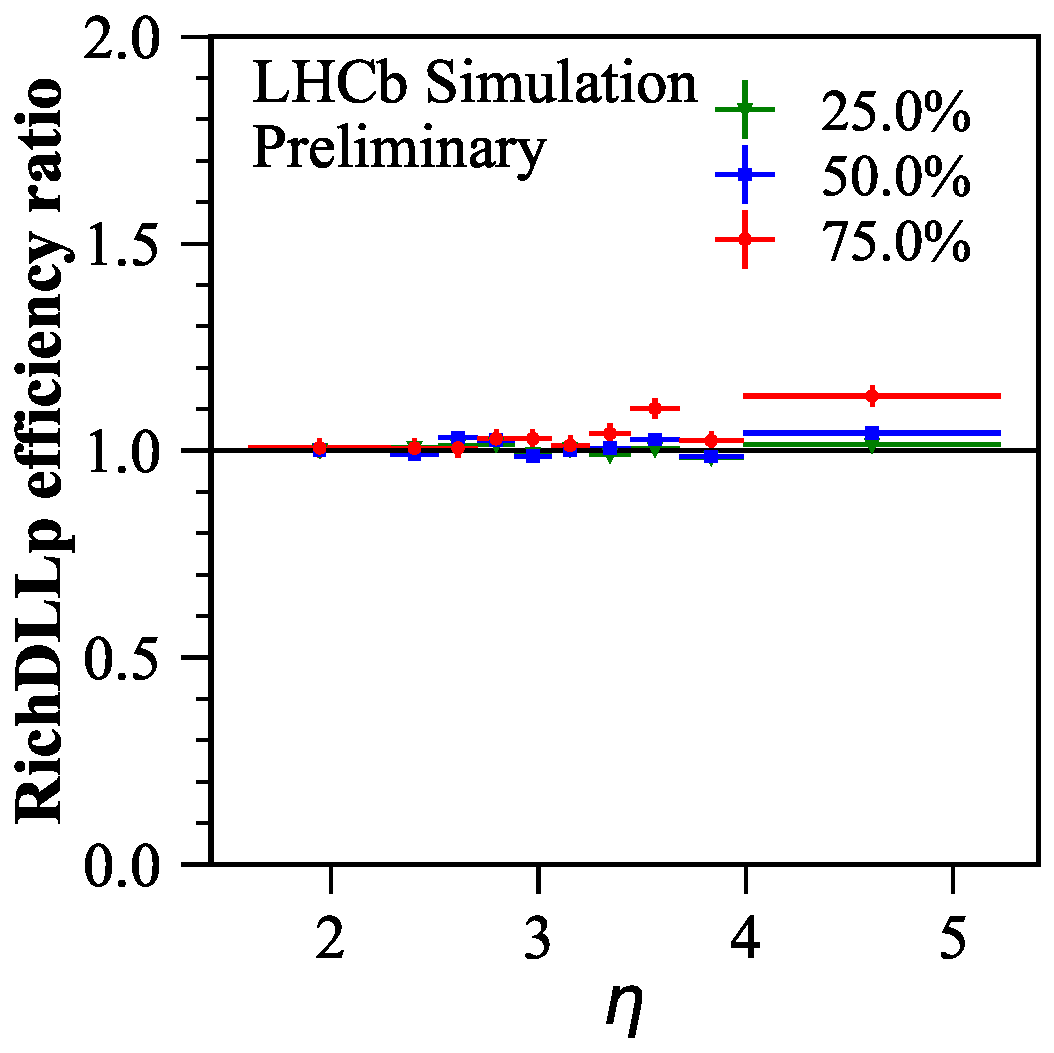
\includegraphics[width=0.32\linewidth]{eff_ratio_RichDLLp_vs_Brunel_ETA_at_[0.05, 0.1, 0.25, 0.5, 0.75, 0.9, 0.95].pdf} &
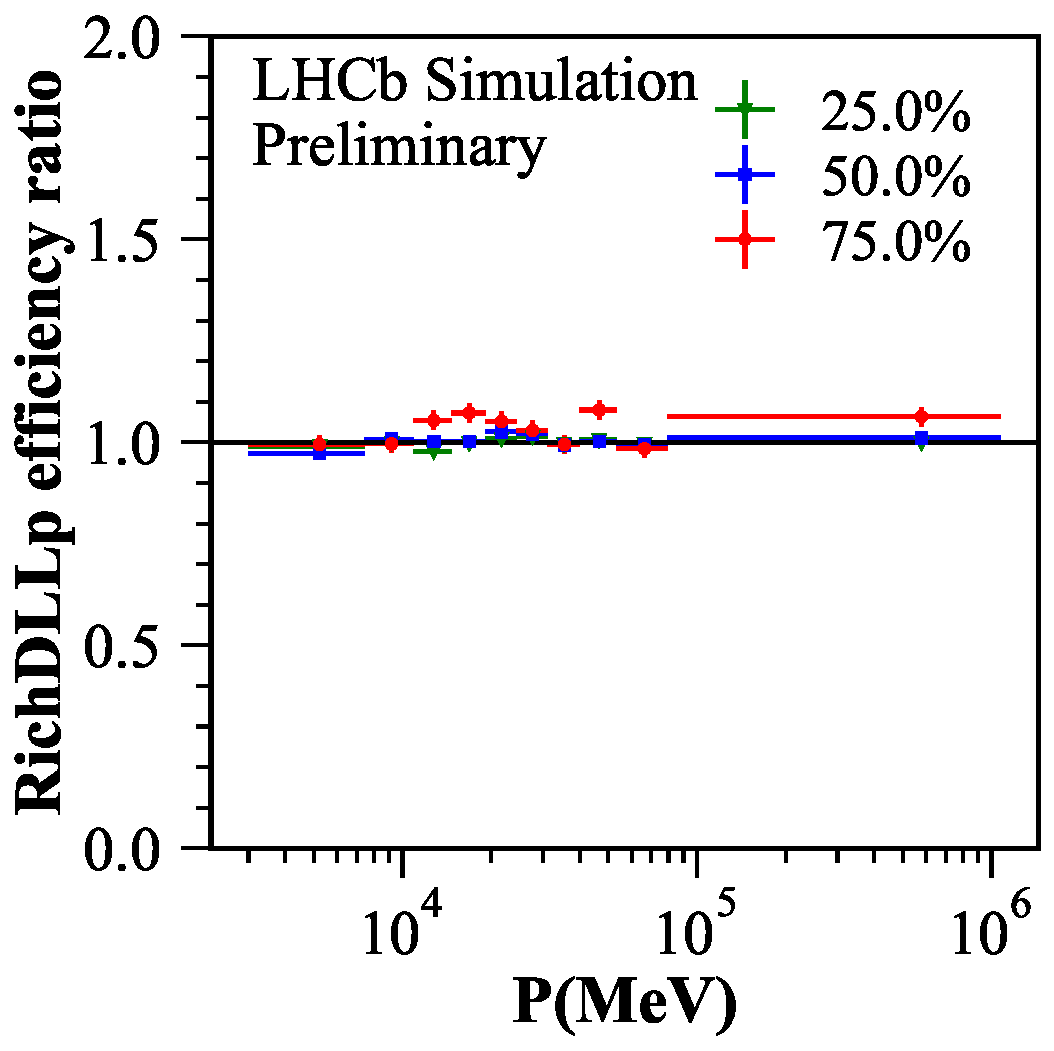
\includegraphics[width=0.32\linewidth]{eff_ratio_RichDLLp_vs_Brunel_P_at_[0.05, 0.1, 0.25, 0.5, 0.75, 0.9, 0.95].pdf} &
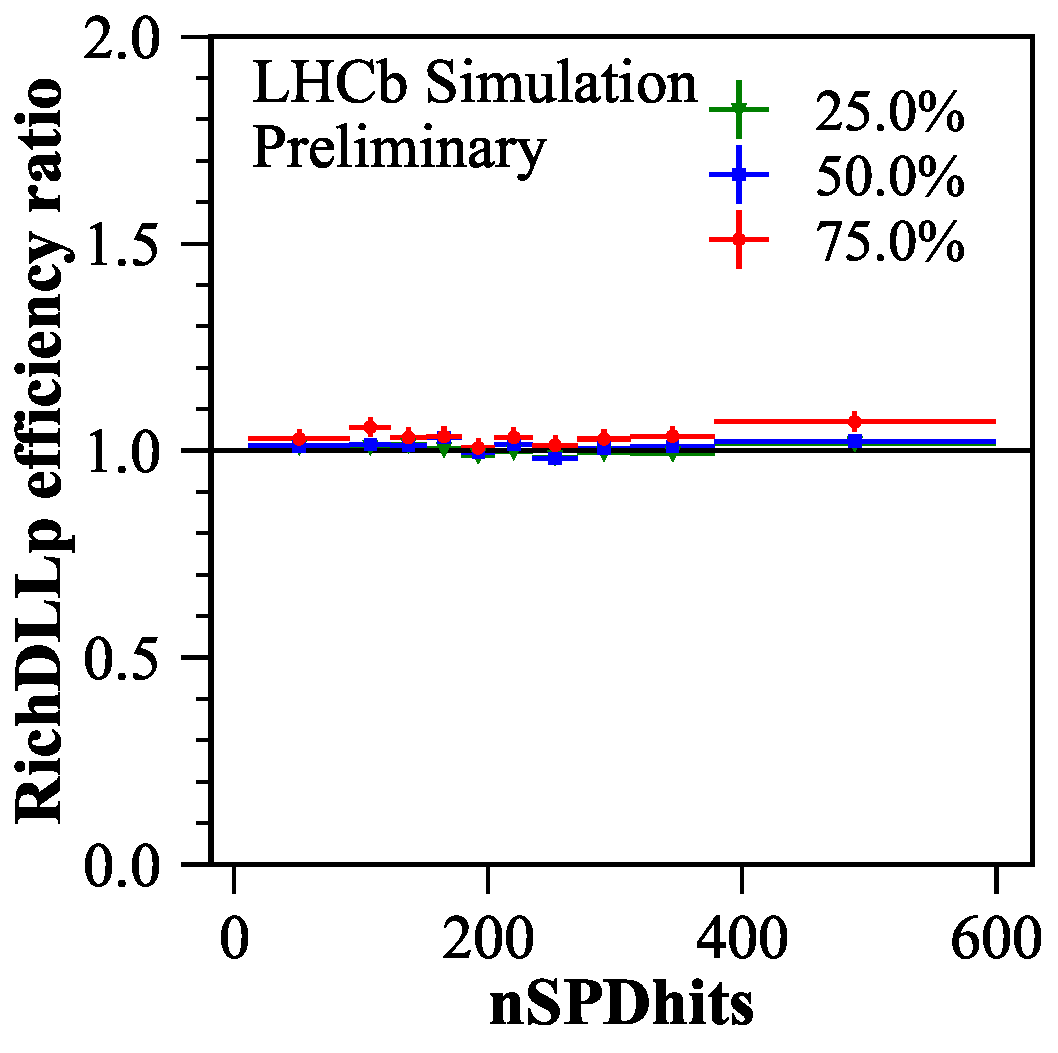
\includegraphics[width=0.32\linewidth]{eff_ratio_RichDLLp_vs_nSPDhits_at_[0.05, 0.1, 0.25, 0.5, 0.75, 0.9, 0.95].pdf}  &
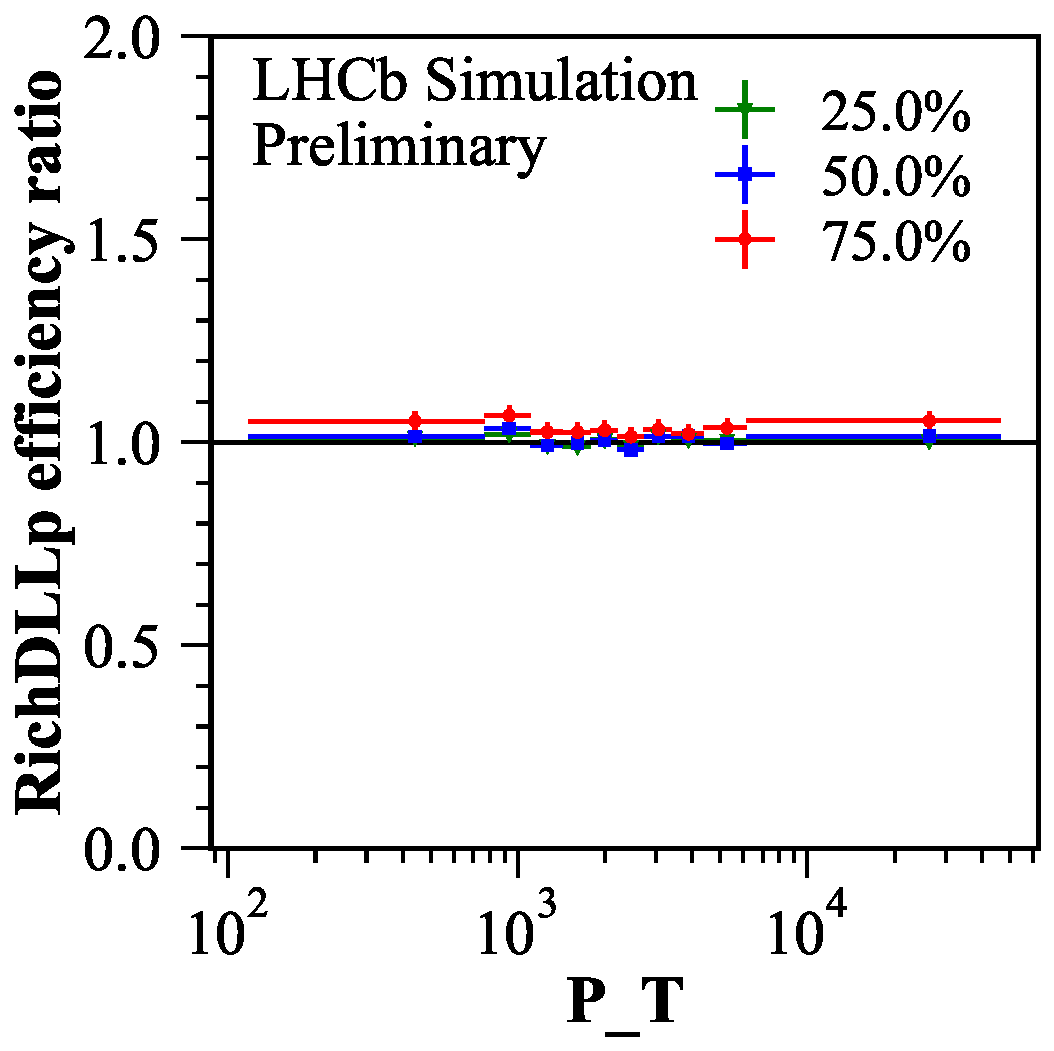
\includegraphics[width=0.32\linewidth]{eff_ratio_RichDLLp_vs_P_T_at_[0.05, 0.1, 0.25, 0.5, 0.75, 0.9, 0.95].pdf}\\
\vspace{-0.2cm}
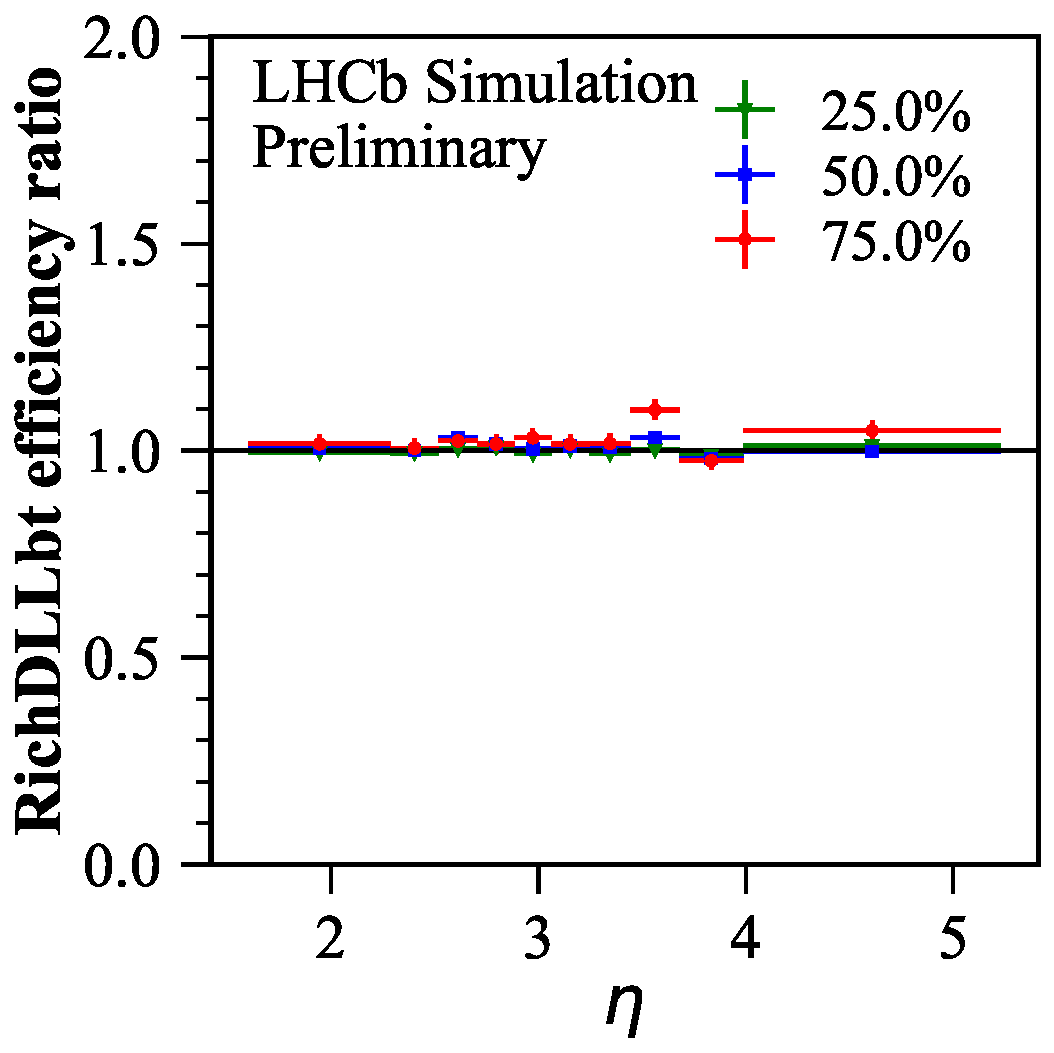
\includegraphics[width=0.32\linewidth]{eff_ratio_RichDLLbt_vs_Brunel_ETA_at_[0.05, 0.1, 0.25, 0.5, 0.75, 0.9, 0.95].pdf} &
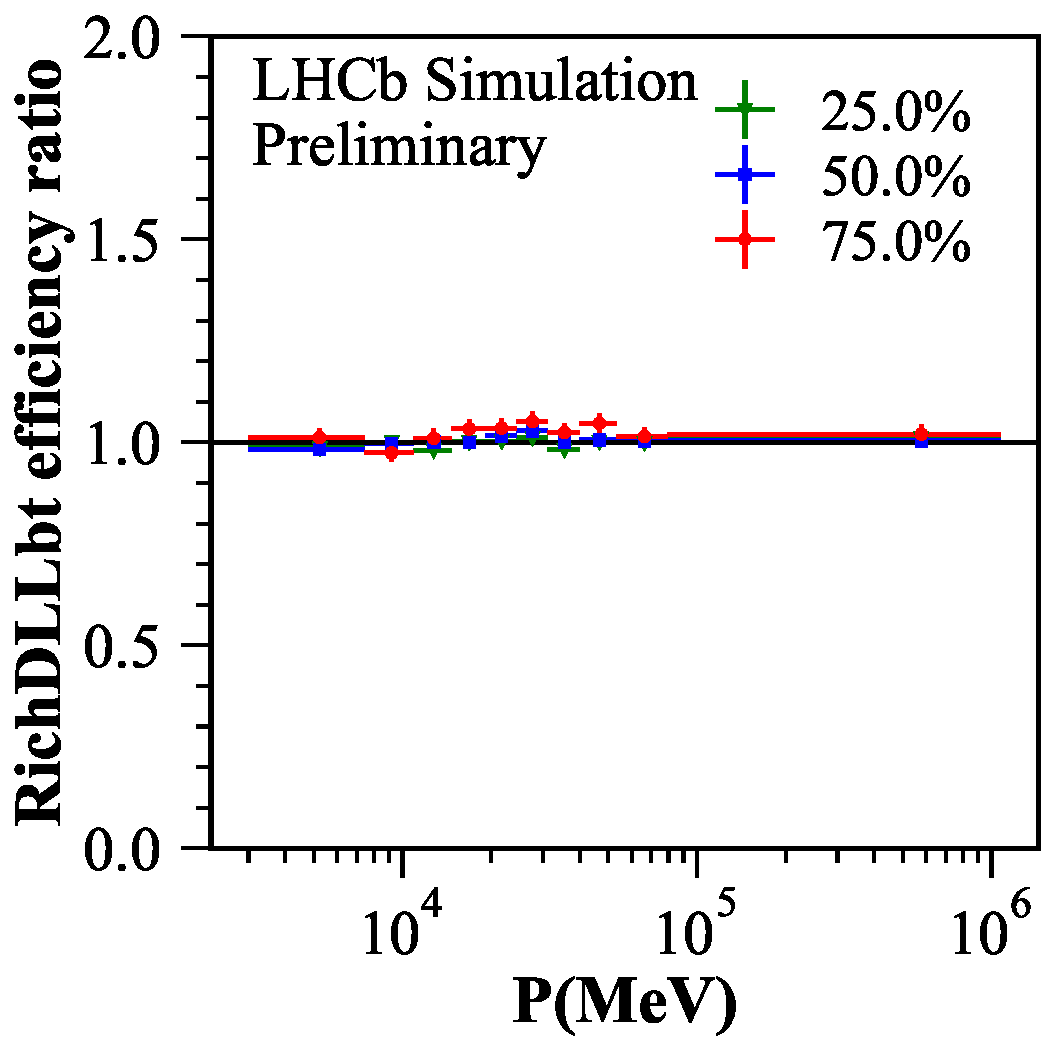
\includegraphics[width=0.32\linewidth]{eff_ratio_RichDLLbt_vs_Brunel_P_at_[0.05, 0.1, 0.25, 0.5, 0.75, 0.9, 0.95].pdf} &
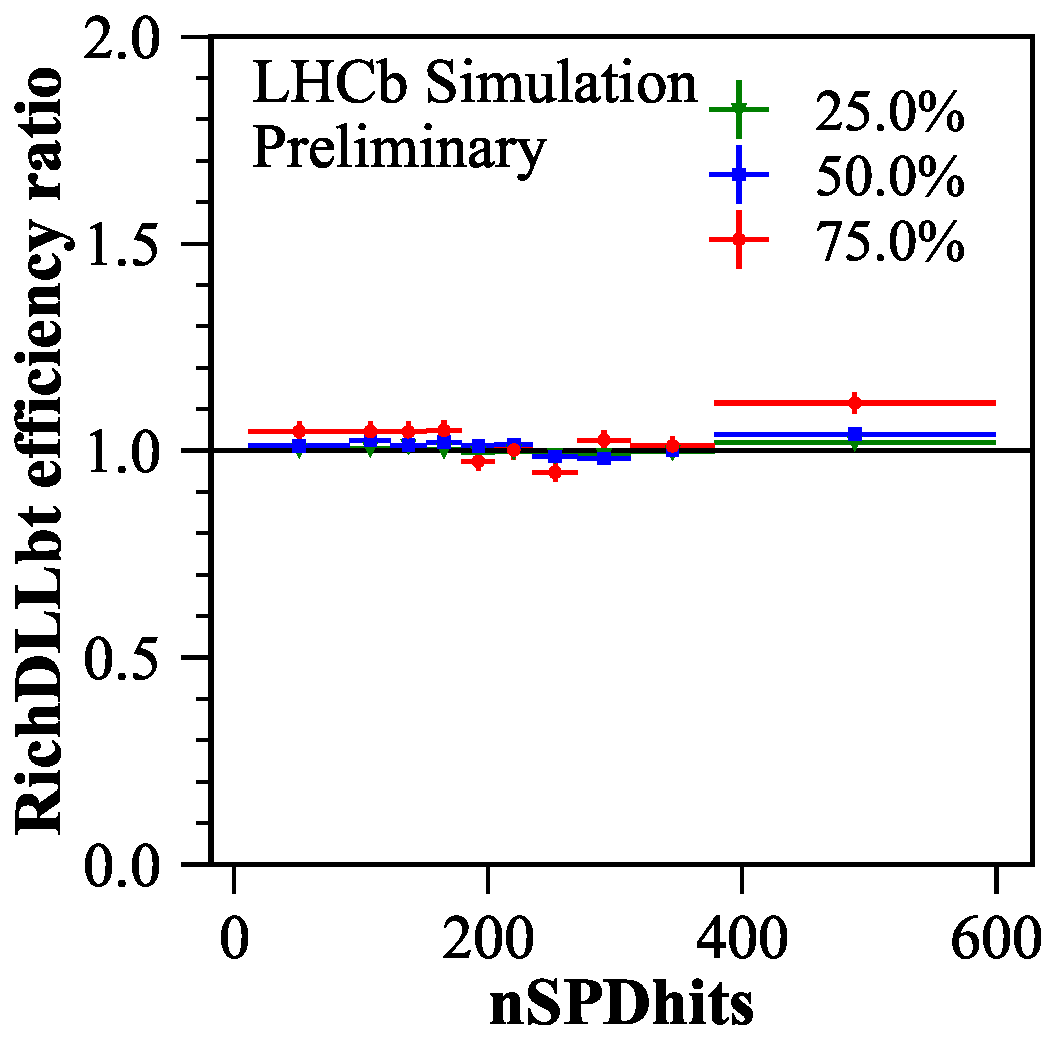
\includegraphics[width=0.32\linewidth]{eff_ratio_RichDLLbt_vs_nSPDhits_at_[0.05, 0.1, 0.25, 0.5, 0.75, 0.9, 0.95].pdf} &
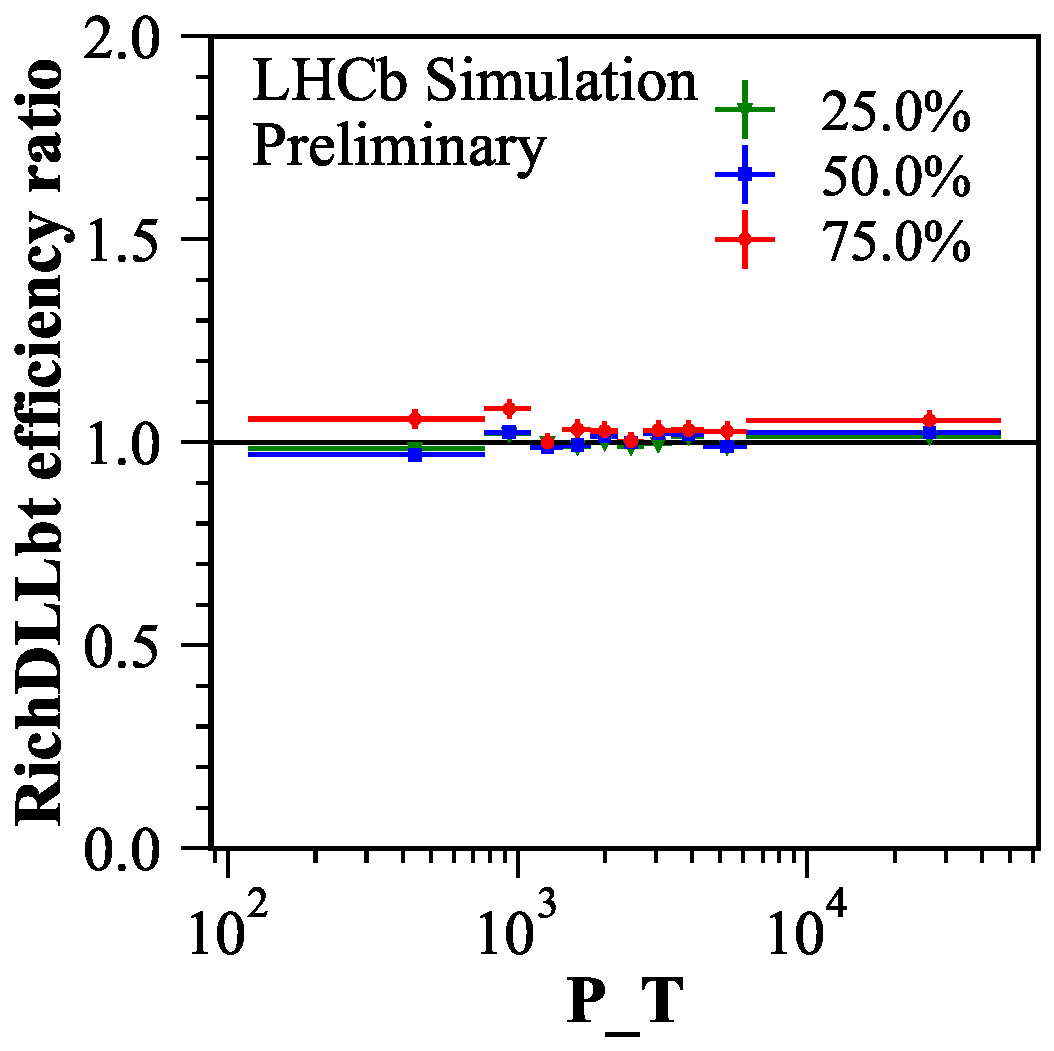
\includegraphics[width=0.32\linewidth]{eff_ratio_RichDLLbt_vs_P_T_at_[0.05, 0.1, 0.25, 0.5, 0.75, 0.9, 0.95].pdf}\\
\vspace{-0.2cm}
\end{tabular}

\end{document}

